
\section{Cyclotron Irradiated Iron}

\subsection{Cyclotron Beam Line}

The Scanditronix MC40 Cyclotron at the University of Birmingham has several beamlines and is capable of accelerating protons, deuterons, Helium 3 and Helium 4 and fluxes and energy ranges detailed below.  After running a simulation with SRIM, the 36MeV protons were expected to create an average of 15.8 vacancies each.

\begin{table}[h]
\begin{center}
\begin{tabular}{c c c c}
\hline
Particle & Energy (MeV) & Max Current (micro A) & Flux (ions per second)\\
\hline
p & 8-40 & 60 & $3.75 \times 10^14$ \\
d & 8-40 & 30 & $1.87 \times 10^14$ \\
${}^4 He^{2+}$ & 8-53 & 30 & $9.36 \times 10^13$ \\
${}^3 He^{2+}$ & 4-20 & 60 & $1.87 \times 10^14$ \\
\end{tabular}
\end{center}
\caption{Beam Characteristics of the Scanditronix MC-40}
\end{table}

The iron sample was held perpendicular to the beam line, with the ions passing through the 0.5mm thickness of the sheet.  The beam area was approximately $6.4 \times 10^{-5} m^2$, irradiating a volume of approximately $3.2 \times 10^{-8} m^3$.  The beam, irradiating the taget for 300 seconds at 0.5 micro amps was expected to cause over $1.4 \times 10^16$ displacements within the volume of iron targetted by the beam.  With a number density of approximately $8\times10^28$ atoms per cubic meter, giving a relatively low damage dose, when compared to that expected over the lifetime of a component within the reactor, of $5 \time 10^{-6}$ DPA.

\begin{figure}[htp]
  \begin{center}
    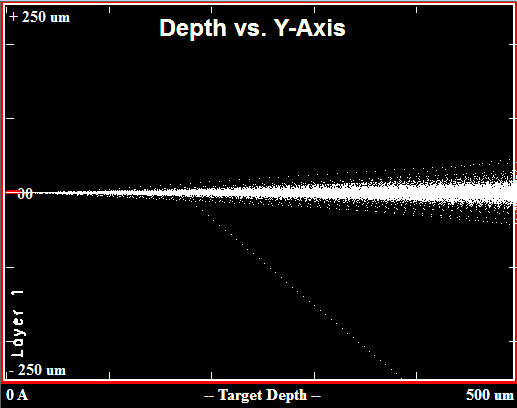
\includegraphics[scale=0.55]{chapters/methodology_activity/images/ion_transport.png}
    \caption{36MeV Ion Track}
    \label{graph:graph1}
  \end{center}
\end{figure}

During irradiation, the amount of Gamma radiation released was enough to trip the alarm for the room.  The proton fluence was less than 1% of the maximum fluence capable of being produced by the cyclotron, so this was definitely a concern.  To increase the damage dose, and keep to a shorter period of time, the current would most probably be increased to a much higher percentage, also increasing the rate of Gammas produced during irradiation.


\subsection{Measurement of Sample Activity}

The sample was too radioactive to safely handle immediately after irradiation, so it was left to cool for several days before taking measurements.









